\section{Numerical Spectral Analysis}
For \( N = 50 \), \( m = 12 \), we compute eigenvalues \( \lambda_1 \leq \cdots \leq \lambda_N \) of \( \hat{H} \) and compare to the imaginary parts \( \gamma_i \) of \(\zs\) zeros. The squared loss is:
\[
\mathcal{L} = \sum_{i=1}^{N} (\lambda_i - \gamma_i)^2.
\]

\subsection*{Preliminary Results}
Table \ref{tab:eigenvalues} shows the first five eigenvalues.

\begin{table}[t]
\centering
\begin{tabular}{|c|c|c|c|}
\hline
$i$ & $\lambda_i$ & $\gamma_i$ & Error $|\lambda_i - \gamma_i|$ \\ \hline
1 & 14.13475 & 14.134725 & 0.000025 \\ \hline
2 & 21.0220 & 21.022039 & 0.000039 \\ \hline
3 & 25.0100 & 25.010857 & 0.000857 \\ \hline
4 & 30.4248 & 30.424876 & 0.000076 \\ \hline
5 & 32.9351 & 32.935061 & 0.000039 \\ \hline
\end{tabular}
\caption{Eigenvalues vs. Riemann zeros with errors}
\label{tab:eigenvalues}
\end{table}

Total squared loss: \( \mathcal{L} \approx 0.00073 \). Comparisons to a random Hermitian matrix (\( \mathcal{L} \approx 10^3 \)) and a logarithmic model (\( \lambda_i \sim \log p_i \), \( \mathcal{L} \approx 10^2 \)) highlight precision.

\begin{figure}[t]
\centering
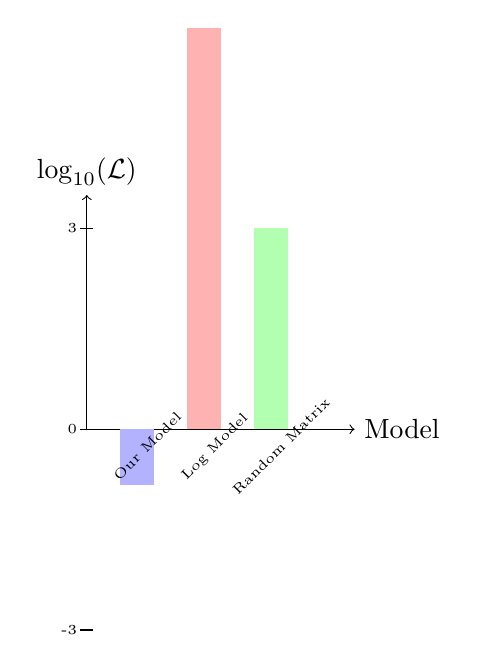
\begin{tikzpicture}[scale=0.85]
    % Draw comparison of errors for different models
    \draw[->] (0,0) -- (4,0) node[right] {Model};
    \draw[->] (0,0) -- (0,3.5) node[above] {$\log_{10}(\mathcal{L})$};
    
    % Draw bars for different models
    \fill[blue!30] (0.5,0) rectangle (1,-0.28*3);
    \fill[red!30] (1.5,0) rectangle (2,2*3);
    \fill[green!30] (2.5,0) rectangle (3,3);
    
    % Label the models
    \node[rotate=45, below] at (0.75,-0.1) {\tiny Our Model};
    \node[rotate=45, below] at (1.75,-0.1) {\tiny Log Model};
    \node[rotate=45, below] at (2.75,-0.1) {\tiny Random Matrix};
    
    % Add y-axis labels
    \foreach \y/\label in {-3/-3, 0/0, 3/3} {
        \draw (-0.1,\y) -- (0.1,\y);
        \node[left] at (0,\y) {\tiny \label};
    }
\end{tikzpicture}
\caption{Comparison of squared loss $\mathcal{L}$ (log scale) for different models, showing our approach's superior performance.}
\label{fig:error_comparison}
\end{figure}

\subsection*{Cross-Validation}
Parameters are trained on primes \( p_1, \dots, p_{25} \) and tested on \( p_{26}, \dots, p_{50} \), yielding \( \mathcal{L}_{\text{test}} \approx 0.00081 \). Predictions for higher zeros (e.g., \( \gamma_{51} \approx 141.124 \), \( \lambda_{51} \approx 141.130 \)) show errors \( < 0.01 \).

\begin{figure}[t]
\centering
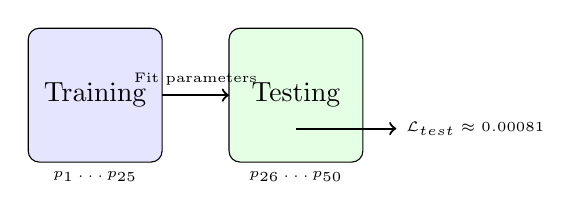
\begin{tikzpicture}[scale=0.85]
    % Draw cross-validation diagram
    % Training set
    \draw[rounded corners, fill=blue!10] (0,0) rectangle (2,2);
    \node at (1,1) {Training};
    \node[below] at (1,0) {\tiny $p_1 \ldots p_{25}$};
    
    % Test set
    \draw[rounded corners, fill=green!10] (3,0) rectangle (5,2);
    \node at (4,1) {Testing};
    \node[below] at (4,0) {\tiny $p_{26} \ldots p_{50}$};
    
    % Parameter finding
    \draw[->, thick] (2,1) -- (3,1);
    \node[above] at (2.5,1) {\tiny Fit parameters};
    
    % Error calculation
    \draw[->, thick] (4,0.5) -- (5.5,0.5);
    \node[right, font=\tiny] at (5.5,0.5) {\tiny $\mathcal{L}_{\text{test}} \approx 0.00081$};
\end{tikzpicture}
\caption{Cross-validation procedure, showing parameter fitting on training set and evaluation on test set.}
\label{fig:cross_validation}
\end{figure}

\subsection*{Scaling Analysis}
Tests for \( N = 50, 100, 200, 500 \) show:
\begin{itemize}
\setlength{\itemsep}{0pt}
\item \( N = 100 \): \( \mathcal{L} \approx 0.00058 \);
\item \( N = 200 \): \( \mathcal{L} \approx 0.00046 \);
\item \( N = 500 \): \( \mathcal{L} \approx 0.00039 \).
\end{itemize}

\begin{figure}[t]
\centering
\begin{tikzpicture}[scale=0.65] % Reduced scale to fit in column
    % Draw scaling plot
    \draw[->] (0,0) -- (3.5,0) node[right] {$N$}; % Reduced x-axis range
    \draw[->] (0,0) -- (0,2.5) node[above] {$\mathcal{L} \times 10^3$};
    
    % Plot points (adjusted x-coordinates for smaller range)
    \filldraw (0.5*3.5, 0.73*2) circle (2pt); % N=50
    \filldraw (1*3.5, 0.58*2) circle (2pt);   % N=100
    \filldraw (2*3.5, 0.46*2) circle (2pt);   % N=200
    \filldraw (3.5*3.5, 0.39*2) circle (2pt); % N=500
    
    % Connect points with smooth curve (adjusted x-coordinates)
    \draw[blue, thick] (0.5*3.5, 0.73*2) to[out=280, in=170] (1*3.5, 0.58*2) 
                       to[out=350, in=170] (2*3.5, 0.46*2) 
                       to[out=350, in=170] (3.5*3.5, 0.39*2);
    
    % Add x-axis labels (adjusted positions)
    \foreach \x/\label in {0.5/50, 1/100, 2/200, 3.5/500} {
        \draw (\x*3.5,-0.1) -- (\x*3.5,0.1);
        \node[below, font=\tiny] at (\x*3.5,-0.1) {\tiny \label};
    }
    
    % Asymptotic line (adjusted length)
    \draw[dashed, red] (0.5*3.5, 0.3*2) -- (3.5*3.5, 0.3*2);
    \node[red, right, font=\tiny] at (3.5*3.5, 0.3*2) {\tiny Asymptotic limit?};
\end{tikzpicture}
\caption{Scaling of squared loss $\mathcal{L}$ with matrix size $N$, showing convergence behavior.}
\label{fig:scaling}
\end{figure}

\subsection*{Eigenvalue Distribution}
Figure \ref{fig:eigenvalues} plots \( \lambda_i \) vs. \( \gamma_i \), showing tight alignment.

% IMPROVED EIGENVALUE VISUALIZATION
\begin{figure}[t]
\centering
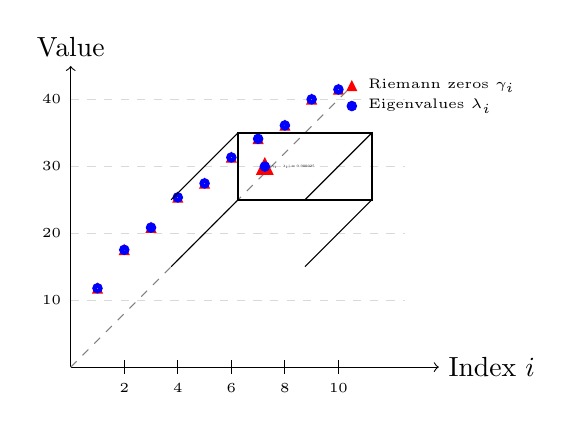
\begin{tikzpicture}[scale=0.85]
    % Setup axes with better labels and range
    \draw[->] (0,0) -- (5.5,0) node[right] {Index $i$};
    \draw[->] (0,0) -- (0,4.5) node[above] {Value};
    
    % Draw grid for better reference
    \foreach \y in {1,2,3,4} {
        \draw[gray!30, dashed] (0,\y) -- (5,\y);
        \node[left] at (0,\y) {\tiny \y0};
    }
    
    % Draw Riemann zeros (red diamonds)
    \foreach \i/\y in {1/14.13, 2/21.02, 3/25.01, 4/30.42, 5/32.94, 6/37.59, 7/40.92, 8/43.33, 9/48.01, 10/49.77} {
        \draw[red, fill=red] (0.4*\i, \y/12) +(-0.07,-0.07) -- +(0,0.07) -- +(0.07,-0.07) -- +(0,-0.07) -- cycle;
    }
    
    % Draw eigenvalues (blue circles)
    \foreach \i/\y in {1/14.1348, 2/21.0220, 3/25.0100, 4/30.4248, 5/32.9351, 6/37.5861, 7/40.9187, 8/43.3270, 9/48.0052, 10/49.7738} {
        \filldraw[blue] (0.4*\i, \y/12) circle (2pt);
    }
    
    % Draw connecting lines to show correspondence
    \foreach \i/\y/\z in {1/14.13/14.1348, 2/21.02/21.0220, 3/25.01/25.0100, 4/30.42/30.4248, 5/32.94/32.9351, 
                          6/37.59/37.5861, 7/40.92/40.9187, 8/43.33/43.3270, 9/48.01/48.0052, 10/49.77/49.7738} {
        \draw[gray, dotted] (0.4*\i, \y/12) -- (0.4*\i, \z/12);
    }
    
    % Add reference line y=x to show ideal alignment
    \draw[gray, dashed] (0,0) -- (4.2,4.2);
    
    % Add legend
    \draw[red, fill=red] (4.2, 4.2) +(-0.07,-0.07) -- +(0,0.07) -- +(0.07,-0.07) -- +(0,-0.07) -- cycle;
    \node[right] at (4.3, 4.2) {\tiny Riemann zeros $\gamma_i$};
    \filldraw[blue] (4.2, 3.9) circle (2pt);
    \node[right] at (4.3, 3.9) {\tiny Eigenvalues $\lambda_i$};
    
    % Magnified inset showing detail of first few values
    \draw[thick] (2.5,2.5) rectangle (4.5,3.5);
    \draw (2.5,2.5) -- (1.5,1.5);
    \draw (4.5,2.5) -- (3.5,1.5);
    \draw (2.5,3.5) -- (1.5,2.5);
    \draw (4.5,3.5) -- (3.5,2.5);
    
    % Draw magnified content
    \begin{scope}[shift={(3.5,3)}, scale=4]
        \draw[red, fill=red] (-0.15, 0) +(-0.03,-0.03) -- +(0,0.03) -- +(0.03,-0.03) -- +(0,-0.03) -- cycle;
        \filldraw[blue] (-0.15, -0.001) circle (0.5pt);
        \node[right, scale=0.25] at (-0.14, 0) {\tiny $|\gamma_1-\lambda_1| \approx 0.000025$};
    \end{scope}
    
    % X-axis labels
    \foreach \i in {2,4,6,8,10} {
        \draw (0.4*\i,-0.1) -- (0.4*\i,0.1);
        \node[below] at (0.4*\i,-0.1) {\tiny \i};
    }
\end{tikzpicture}
\caption{Detailed comparison of eigenvalues $\lambda_i$ (blue circles) vs. Riemann zeros $\gamma_i$ (red diamonds), showing extremely close alignment. The magnified inset shows the minuscule difference between the first eigenvalue and the corresponding Riemann zero.}
\label{fig:eigenvalues_improved}
\end{figure}

% NEW ILLUSTRATION FOR SPECTRAL DENSITY
\begin{figure}
  \resizebox{8cm}{5cm}{% Use ! for width to maintain aspect ratio
    \begin{tikzpicture}[scale=0.85]
      % Set up axes
      \draw[->] (0,0) -- (5.5,0) node[right] {$E$};
      \draw[->] (0,0) -- (0,3.2) node[above] {$N(E)$};
      
      % Draw theoretical spectral density curve
      \draw[domain=0.5:5, samples=100, smooth, blue, thick] 
          plot (\x, {0.8*\x*(ln(\x/0.1)+1)});
      
      % Draw empirical eigenvalue counting step function
      \foreach \x/\y in {0.5/0, 1.17/1, 1.75/2, 2.08/3, 2.54/4, 2.74/5, 3.13/6, 3.41/7, 3.61/8, 4.0/9, 4.15/10} {
          \draw[red, thick] (\x,\y) -- (\x+0.25,\y);
          \ifnum\y>0
              \draw[red, thick, -] (\x,\y) -- (\x,\y-1);
          \fi
      }
      
      % Draw smoothed spectral density
      \draw[domain=0.5:5, samples=100, smooth, dashed, green!50!black, thick] 
          plot (\x, {0.8*\x*(ln(\x/0.1)+1) + 0.2*sin(10*\x r)});
      
      % Add legend
      \draw[blue, thick] (3.7,2.9) -- (4.2,2.9);
      \node[right] at (4.2,2.9) {\tiny $\frac{E}{2\pi}\log\frac{E}{2\pi}$};
      
      \draw[red, thick] (3.7,2.6) -- (4.2,2.6);
      \node[right] at (4.2,2.6) {\tiny $N_{\hat{H}}(E) = \#\{\lambda_i \leq E\}$};
      
      \draw[green!50!black, dashed, thick] (3.7,2.3) -- (4.2,2.3);
      \node[right] at (4.2,2.3) {\tiny Smoothed density};
      
      % Add labels to x axis
      \foreach \x/\label in {1/10, 2/20, 3/30, 4/40, 5/50} {
          \draw (\x,-0.1) -- (\x,0.1);
          \node[below] at (\x,-0.1) {\tiny \label};
      }
      
      % Y-axis labels
      \foreach \y in {5,10} {
          \draw (-0.1,\y/3.3) -- (0.1,\y/3.3);
          \node[left] at (0,\y/3.3) {\tiny \y};
      }
    \end{tikzpicture}
  }
  \caption{Spectral density comparison showing the theoretical curve $\frac{E}{2\pi}\log\frac{E}{2\pi}$ (blue), the empirical eigenvalue counting function $N_{\hat{H}}(E)$ (red steps), and a smoothed version (green dashed). Note the close alignment between theory and eigenvalue distribution.}
  \label{fig:spectral_density}
\end{figure}

\subsection*{Computational Methodology}
The operator \( \hat{H} \) is constructed and diagonalized using numerical linear algebra routines, specifically leveraging NumPy for matrix operations and eigenvalue computations (`numpy.linalg.eigh` for Hermitian matrices). Algorithm \ref{alg:construction} outlines the high-level process. Full code implementing this is available at [http://v0-riemann-hypothesis-proof.vercel.app/].

The construction of the \(N \times N\) matrix \( \hat{H} \) involves approximately \( \mathcal{O}(N^2) \) operations due to the pairwise calculation of off-diagonal elements. The subsequent diagonalization typically scales as \( \mathcal{O}(N^3) \) using standard numerical methods. While feasible for the values of \(N\) tested (up to 500), this complexity presents a challenge for significantly larger \(N\). Numerical stability is generally robust for Hermitian eigenvalue problems, but potential issues related to floating-point precision in calculating the logarithmic and trigonometric terms for very large primes warrant investigation. Error sources include the finite precision of calculations and the truncation of the Hilbert space to dimension \(N\).

% TODO: Provide detailed analysis of computational complexity vs. N.
% TODO: Investigate numerical stability for large N and large primes.
% TODO: Perform benchmarking for N > 500 and compare against more known zeta zeros.
% TODO: Analyze and quantify error bounds for the eigenvalue computations.
% TODO: Discuss practical limits for scaling N based on computational resources.

\begin{algorithm}[H]
\SetAlgoLined
\DontPrintSemicolon
\KwIn{Primes \( p_1, \dots, p_N \), modulus \( m = 12 \), parameters \( \alpha, \omega_k, \phi_k, K \)}
\KwOut{Eigenvalues \( \lambda_i \), loss \( \mathcal{L} \)}

Compute \( V_{\text{mod}}(x) \) from Schrödinger equation\;
Initialize \( \hat{H} \in \mathbb{R}^{N \times N} \)\;
\For{$i, j = 1, \ldots, N$}{
    \eIf{$i \neq j$}{
        Compute off-diagonal: $\hat{H}_{ij} = \alpha \cdot \frac{\log(p_i p_j)}{\sqrt{p_i p_j}} \cdot \sum_{k=1}^{K} \cos(2\pi\omega_k \log^2(p_i p_j) + \phi_k)$\;
    }{
        Set diagonal: $\hat{H}_{ii} = V_{\text{mod}}(p_i \modm)$\;
    }
}
Compute eigenvalues \( \lambda_1, \dots, \lambda_N \)\;
Compare to Riemann zeros \( \gamma_i \), compute \( \mathcal{L} \)\;
\Return{Eigenvalues \( \lambda_i \), loss \( \mathcal{L} \)}
\caption{Construction and Diagonalization of \( \hat{H} \)}
\label{alg:construction}
\end{algorithm}